\documentclass[aspectratio=169]{beamer}

% MicroCD Labs customer intro deck.
% Casual, simple, and matched to the website visual style.
% Compile with: pdflatex customer_intro_deck.tex

\usepackage{graphicx}
\usepackage{tikz}
\usepackage[absolute,overlay]{textpos}

\usetheme{default}
\usefonttheme{professionalfonts}
\setbeamertemplate{navigation symbols}{}
\setbeamertemplate{footline}{%
  \hfill{\scriptsize\color{MicroCDMuted}\insertframenumber/\inserttotalframenumber}\hspace{1em}\vspace{0.6em}
}

\definecolor{MicroCDGreen}{HTML}{0F766E}
\definecolor{MicroCDDark}{HTML}{18211F}
\definecolor{MicroCDMuted}{HTML}{5D6965}
\definecolor{MicroCDSoft}{HTML}{F4F8F6}
\definecolor{MicroCDLine}{HTML}{D9E1DD}
\definecolor{MicroCDCoral}{HTML}{D85B45}
\definecolor{MicroCDAmber}{HTML}{D79A2B}

\setbeamercolor{normal text}{fg=MicroCDDark,bg=white}
\setbeamercolor{frametitle}{fg=MicroCDDark,bg=white}
\setbeamercolor{title}{fg=white}
\setbeamercolor{subtitle}{fg=white}
\setbeamercolor{structure}{fg=MicroCDGreen}
\setbeamercolor{itemize item}{fg=MicroCDGreen}
\setbeamercolor{enumerate item}{fg=MicroCDGreen}

\setbeamerfont{title}{size=\Huge,series=\bfseries}
\setbeamerfont{subtitle}{size=\large}
\setbeamerfont{frametitle}{size=\Large,series=\bfseries}

\setlength{\parindent}{0pt}
\setlength{\parskip}{0.45em}

\newcommand{\eyebrow}[1]{%
  {\footnotesize\bfseries\color{MicroCDCoral}\MakeUppercase{#1}}\vspace{0.55em}
}

\newcommand{\muted}[1]{%
  {\color{MicroCDMuted}#1}
}

\newcommand{\sitecard}[3]{%
  \begin{minipage}[t]{0.31\textwidth}
    \setlength{\fboxsep}{0pt}%
    \colorbox{MicroCDSoft}{%
      \begin{minipage}[t][0.31\textheight][t]{\linewidth}
        \includegraphics[width=\linewidth,height=0.135\textheight]{#1}
        \vspace{0.55em}
        \hspace{0.65em}\begin{minipage}{0.86\linewidth}
          {\bfseries #2}

          {\footnotesize\color{MicroCDMuted}#3}
        \end{minipage}
      \end{minipage}
    }
  \end{minipage}
}

\newcommand{\widephoto}[1]{%
  \includegraphics[width=\linewidth,height=0.54\textheight]{#1}
}

\newcommand{\pill}[1]{%
  \tikz[baseline=(text.base)]{
    \node[
      fill=MicroCDSoft,
      draw=MicroCDGreen!20,
      rounded corners=4pt,
      inner xsep=8pt,
      inner ysep=5pt
    ] (text) {\small\bfseries #1};
  }%
}

\newcommand{\roaditem}[3]{%
  \begin{minipage}[t]{0.23\textwidth}
    {\large\bfseries\color{MicroCDGreen}#1}

    \vspace{0.35em}
    {\bfseries #2}

    \vspace{0.25em}
    {\footnotesize\color{MicroCDMuted}#3}
  \end{minipage}
}

\title{MicroCD Labs}
\subtitle{Microfluidics parts, equipment, and practical support for research teams}
\author{Snehan Peshin, Ph.D.}
\date{}

\begin{document}

\begin{frame}[plain]
  \begin{tikzpicture}[remember picture,overlay]
    \node[anchor=center] at (current page.center) {%
      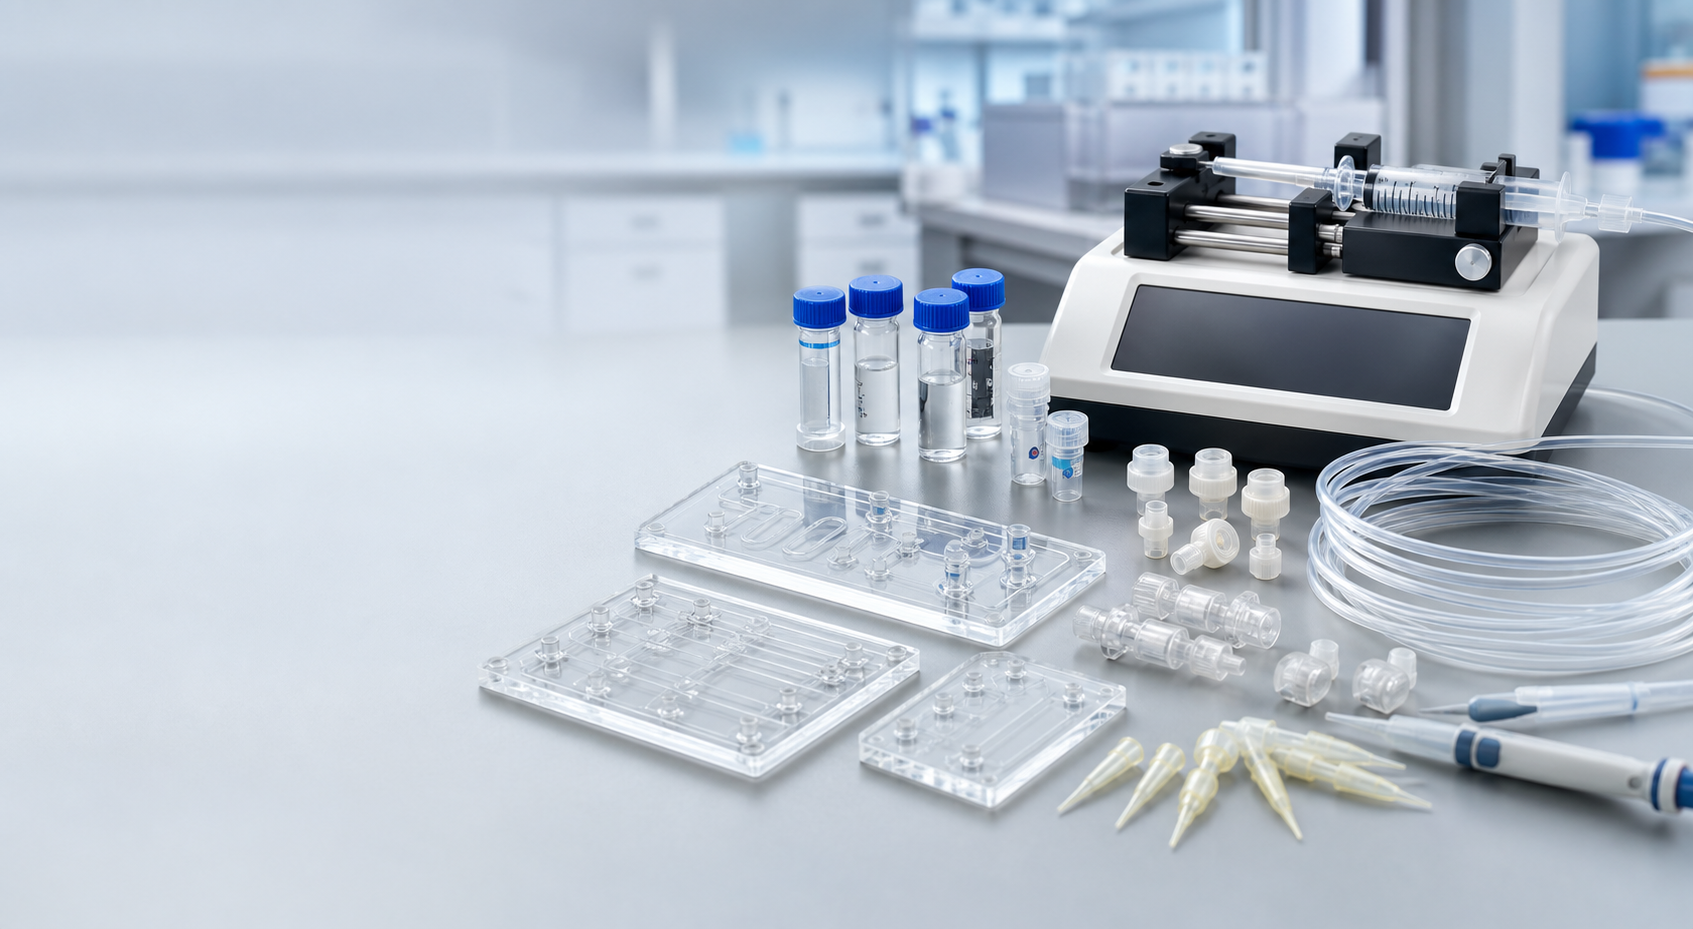
\includegraphics[width=\paperwidth,height=\paperheight]{assets/hero-lab-supply.png}
    };
    \fill[MicroCDDark,opacity=0.74] (current page.south west) rectangle ([xshift=0.58\paperwidth]current page.north west);
    \fill[MicroCDDark,opacity=0.22] ([xshift=0.58\paperwidth]current page.south west) rectangle (current page.north east);
  \end{tikzpicture}

  \vspace{1.8em}
  {\footnotesize\bfseries\color{MicroCDCoral}LONDON-BASED MICROFLUIDICS SUPPLY}

  \vspace{1.1em}
  {\Huge\bfseries\color{white} MicroCD Labs}

  \vspace{0.45em}
  {\Large\color{white} Microfluidic parts and benchtop equipment for R\&D teams.}

  \vspace{1.2em}
  {\normalsize\color{white} Research-use tubing, fittings, plastic connectors, chips, pumps, and starter kits.}

  \vfill
  {\footnotesize\color{white} info@microcdlabs.com \quad | \quad sites.google.com/view/microcd-labs/home}
\end{frame}

\begin{frame}{What we do}
  \eyebrow{Simple sourcing}

  \begin{columns}[T]
    \begin{column}{0.52\textwidth}
      {\Large\bfseries Microfluidics essentials without the supplier maze.}

      \vspace{0.8em}
      \muted{MicroCD Labs helps research teams source the practical parts behind microfluidic experiments, from tubing and fittings to chips, pumps, and starter kits.}

      \vspace{1em}
      \begin{itemize}
        \item Research-use supply
        \item Early feasibility setups
        \item Friendly technical guidance
      \end{itemize}
    \end{column}
    \begin{column}{0.42\textwidth}
      \widephoto{assets/deck-images/microfluidic-device.jpg}
    \end{column}
  \end{columns}
\end{frame}

\begin{frame}{Who we help}
  \eyebrow{Built for labs}

  \sitecard{assets/deck-images/chip.jpg}{University labs}{Small orders, starter setups, repeat supplies, and experiment-specific parts.}
  \hfill
  \sitecard{assets/deck-images/laminar-flow.png}{Biotech teams}{Practical sourcing for assay, diagnostics, and lab-on-chip development.}
  \hfill
  \sitecard{assets/deck-images/syringe-pump.jpg}{R\&D builders}{Parts for prototypes, feasibility studies, and benchtop testing.}

  \vspace{1em}
  \muted{If you know your experiment but not the exact part number, we can still help.}
\end{frame}

\begin{frame}{Starter catalog}
  \eyebrow{Core parts and equipment}

  \begin{columns}[T]
    \begin{column}{0.47\textwidth}
      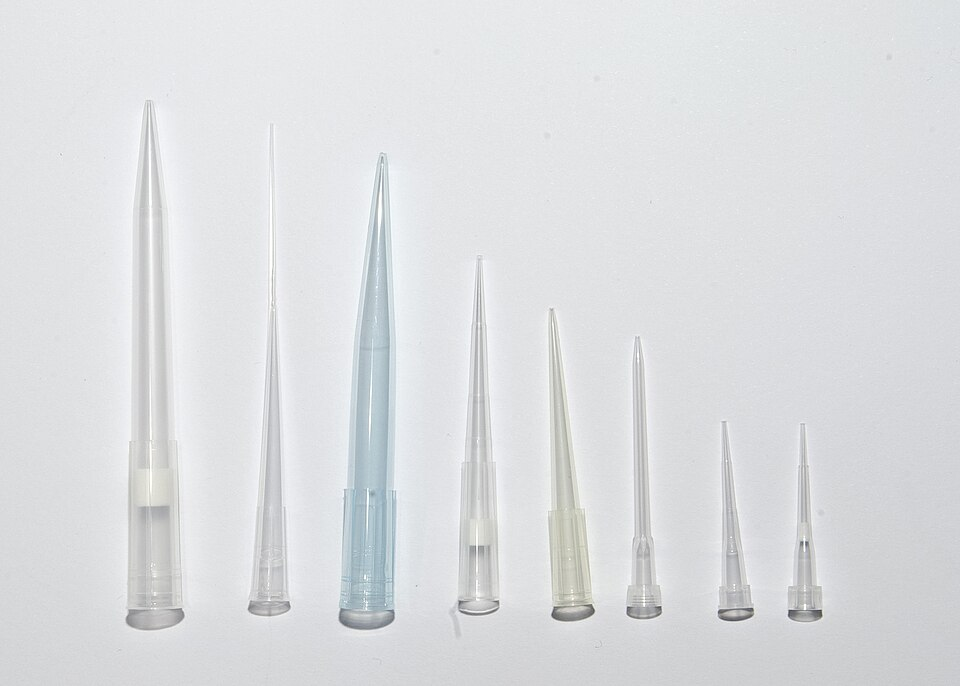
\includegraphics[width=\linewidth,height=0.37\textheight]{assets/deck-images/pipette-tips.jpg}
      \vspace{0.7em}
      \begin{itemize}
        \item Microbore tubing
        \item Luer fittings and connectors
        \item Plastic caps, plugs, clips, ferrules, and adapters
      \end{itemize}
    \end{column}
    \begin{column}{0.47\textwidth}
      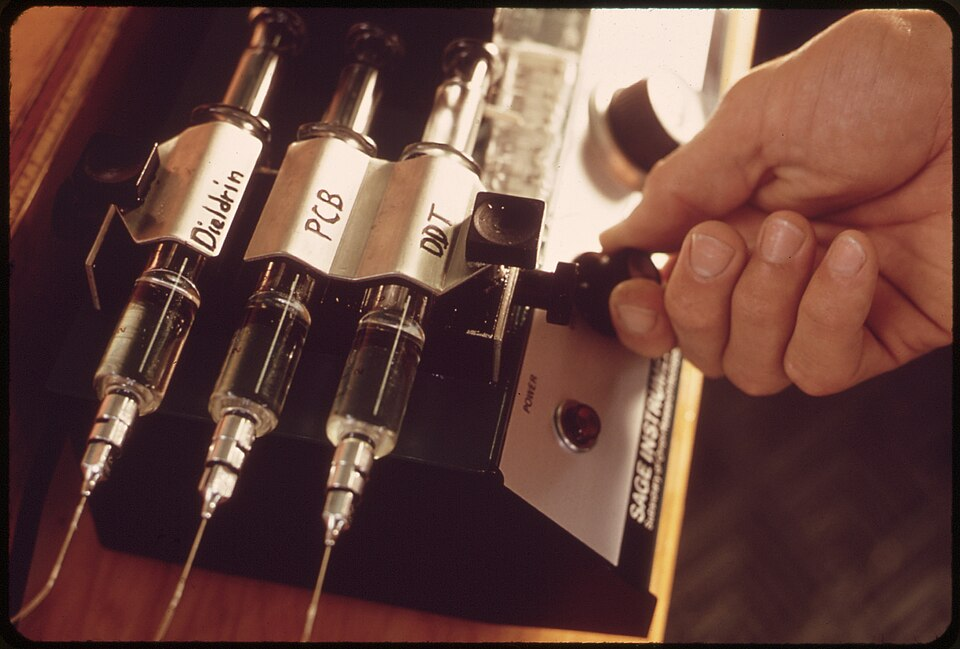
\includegraphics[width=\linewidth,height=0.37\textheight]{assets/deck-images/syringe-pump.jpg}
      \vspace{0.7em}
      \begin{itemize}
        \item Syringe pump options
        \item Low-flow sensor modules
        \item Droplet chips, chip holders, and starter bundles
      \end{itemize}
    \end{column}
  \end{columns}
\end{frame}

\begin{frame}{Founder slide}
  \eyebrow{Scientific and product background}

  \begin{columns}[T]
    \begin{column}{0.52\textwidth}
      {\Large\bfseries Snehan Peshin, Ph.D.}

      \vspace{0.7em}
      \muted{Biomedical R\&D experience across assay development, diagnostics, microfluidics, lab-on-disc systems, and practical product development.}

      \vspace{1em}
      \pill{Ph.D., UC Irvine}\quad
      \pill{Zoetis}

      \vspace{0.65em}
      \pill{BlueJay Diagnostics}\quad
      \pill{Vanderbilt}
    \end{column}
    \begin{column}{0.40\textwidth}
      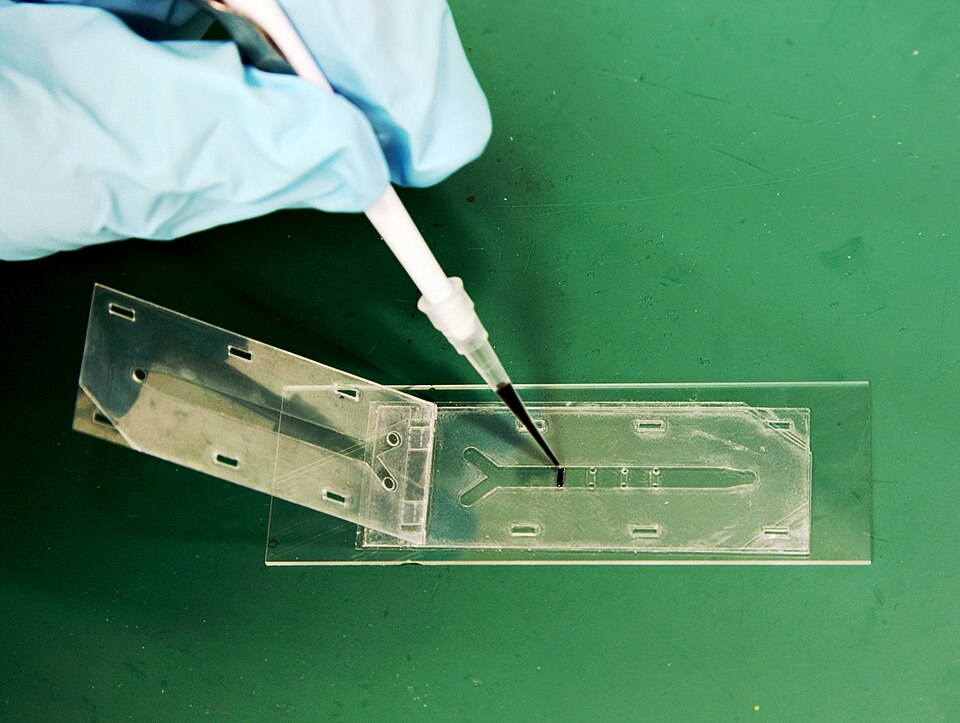
\includegraphics[width=\linewidth,height=0.52\textheight]{assets/deck-images/microfluidic-device.jpg}
    \end{column}
  \end{columns}
\end{frame}

\begin{frame}{Technical expertise}
  \eyebrow{Microfluidics, systems, and integration}

  \begin{columns}[T]
    \begin{column}{0.48\textwidth}
      \begin{itemize}
        \item Lab-on-a-disc workflows
        \item Lab-on-chip architecture
        \item Fluid routing and cartridge concepts
        \item Rapid prototyping and benchtop testing
      \end{itemize}
    \end{column}
    \begin{column}{0.48\textwidth}
      \begin{itemize}
        \item Pump, sensor, and connector selection
        \item Consumable and cartridge thinking
        \item System integration
        \item Early design-for-manufacturing planning
      \end{itemize}
    \end{column}
  \end{columns}

  \vspace{1em}
  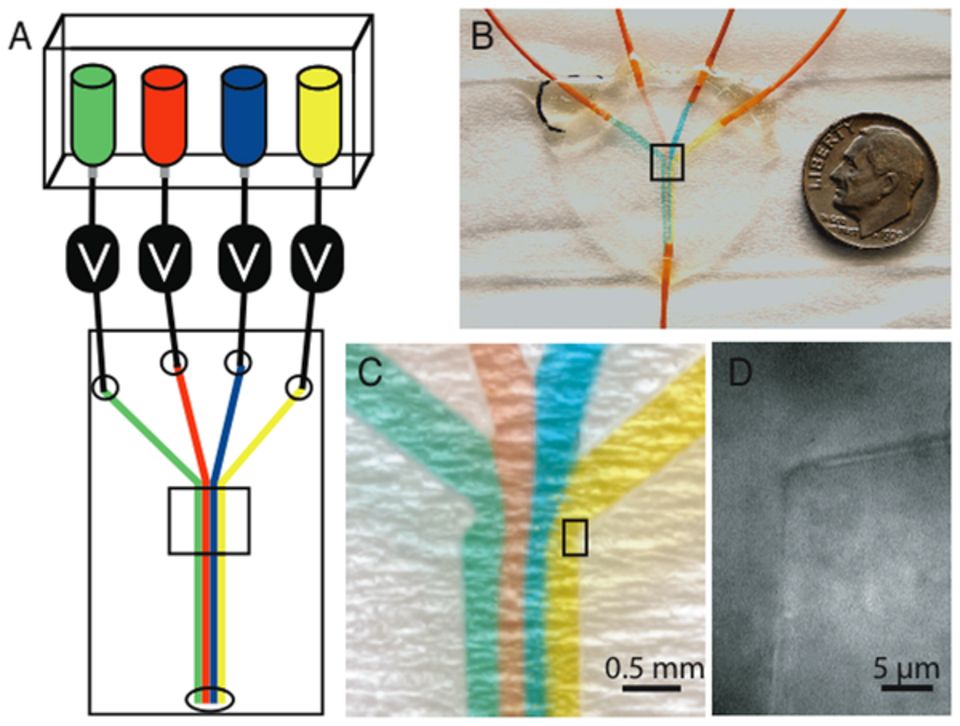
\includegraphics[width=\linewidth,height=0.25\textheight]{assets/deck-images/laminar-flow.png}
\end{frame}

\begin{frame}{Diagnostics and assay-development capabilities}
  \eyebrow{From assay idea to usable workflow}

  \begin{columns}[T]
    \begin{column}{0.52\textwidth}
      {\large\bfseries Core capabilities}

      \begin{itemize}
        \item Assay development and feasibility testing
        \item Diagnostic workflow design
        \item Sample-to-answer thinking
        \item Reagent, fluidic, and consumable constraints
        \item Translation from bench protocol to device workflow
      \end{itemize}
    \end{column}
    \begin{column}{0.40\textwidth}
      \colorbox{MicroCDSoft}{%
        \begin{minipage}[c][0.48\textheight][c]{0.92\linewidth}
          \centering
          {\Large\bfseries Practical diagnostic R\&D}

          \vspace{0.8em}
          \muted{MicroCD Labs can support early-stage assay and microfluidic workflow planning before larger engineering investment.}
        \end{minipage}
      }
    \end{column}
  \end{columns}
\end{frame}

\begin{frame}{Future product roadmap}
  \eyebrow{Near-term supply, long-term product platform}

  \roaditem{01}{Research tools}{Starter kits, fittings, chips, pumps, and useful lab accessories.}
  \hfill
  \roaditem{02}{Custom consumables}{Application-specific parts for pilot studies and repeat research use.}
  \hfill
  \roaditem{03}{OEM cartridges}{Cartridge and consumable concepts for partner assay workflows.}
  \hfill
  \roaditem{04}{POC diagnostics}{Future point-of-care and lab-on-disc diagnostic workflows.}

  \vspace{1.5em}
  \muted{The roadmap starts practical: serve researchers now while building toward higher-value diagnostic and consumable products.}
\end{frame}

\begin{frame}{Partnership opportunities}
  \eyebrow{Where collaboration may help}

  \begin{columns}[T]
    \begin{column}{0.50\textwidth}
      \begin{itemize}
        \item Prototype fabrication partners
        \item Glass and polymer microfluidic manufacturers
        \item Design-for-manufacturing support
        \item Pilot production and small-batch consumables
        \item Academic and biotech assay partners
      \end{itemize}
    \end{column}
    \begin{column}{0.42\textwidth}
      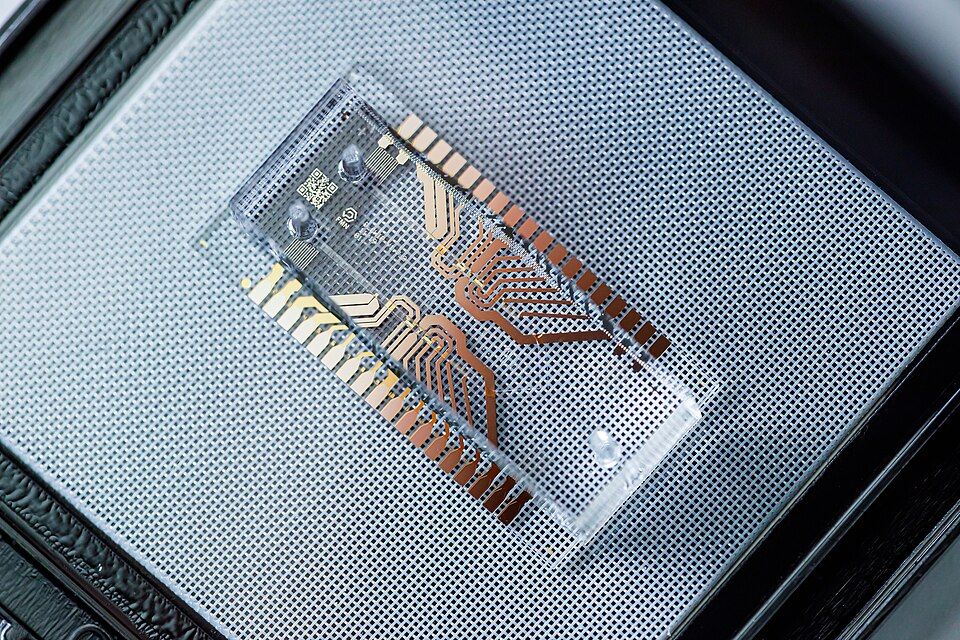
\includegraphics[width=\linewidth,height=0.48\textheight]{assets/deck-images/chip.jpg}
    \end{column}
  \end{columns}

  \vspace{0.6em}
  {\footnotesize\color{MicroCDMuted}Potential collaboration examples include cartridge prototyping, microfluidic design translation, and early pilot manufacturing.}
\end{frame}

\begin{frame}{How a quote works}
  \eyebrow{No complicated ordering flow}

  \begin{columns}[T]
    \begin{column}{0.52\textwidth}
      \begin{enumerate}
        \item Tell us what you are trying to build or test.
        \item Share useful details: tubing size, flow rate, solvent, chip type, or destination country.
        \item We prepare a simple parts list or quote.
        \item You review, ask questions, and order only what makes sense.
      \end{enumerate}
    \end{column}
    \begin{column}{0.40\textwidth}
      \colorbox{MicroCDSoft}{%
        \begin{minipage}[c][0.46\textheight][c]{0.92\linewidth}
          \centering
          {\Large\bfseries Request a quote}

          \vspace{0.8em}
          \muted{Send the parts you need and a few experiment notes.}

          \vspace{1em}
          {\bfseries\color{MicroCDGreen}info@microcdlabs.com}
        \end{minipage}
      }
    \end{column}
  \end{columns}
\end{frame}

\begin{frame}{Why MicroCD Labs}
  \eyebrow{Small, technical, responsive}

  \begin{columns}[T]
    \begin{column}{0.48\textwidth}
      {\large\bfseries Microfluidics background}

      \muted{Built around real lab experience in diagnostics, microfluidics, assays, lab-on-disc work, and practical R\&D.}

      \vspace{1em}
      {\large\bfseries Human help}

      \muted{You can ask a specific technical question and get a practical answer.}
    \end{column}
    \begin{column}{0.45\textwidth}
      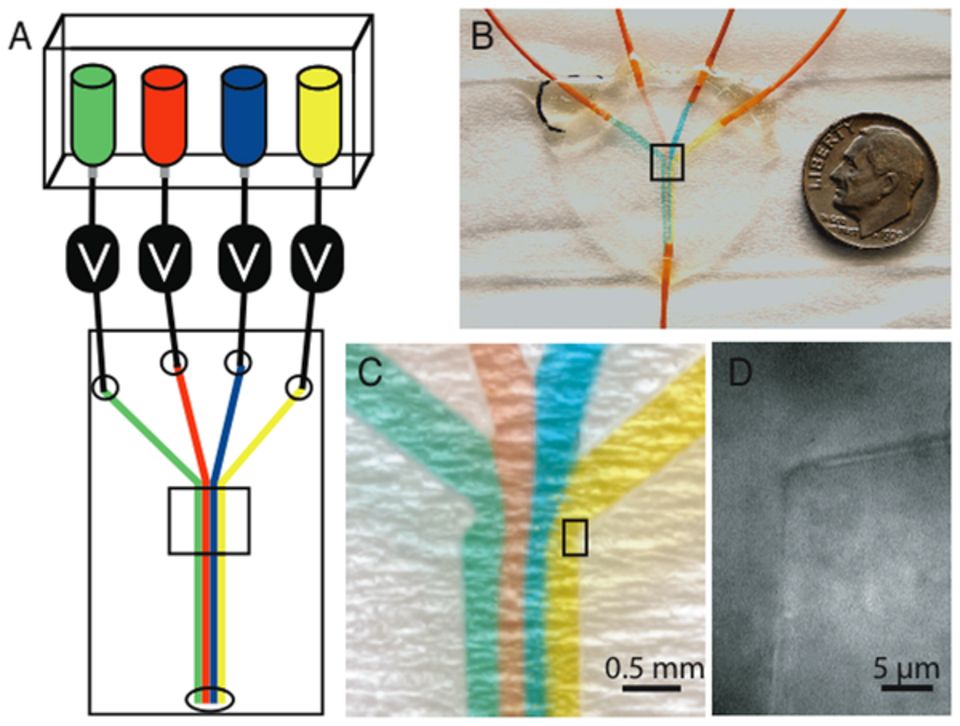
\includegraphics[width=\linewidth,height=0.48\textheight]{assets/deck-images/laminar-flow.png}

      \vspace{0.6em}
      {\footnotesize\color{MicroCDMuted}Research-use products only unless stated otherwise. International requests are reviewed before shipment.}
    \end{column}
  \end{columns}
\end{frame}

\begin{frame}{What to send us}
  \eyebrow{A short message is enough}

  \begin{columns}[T]
    \begin{column}{0.58\textwidth}
      \begin{itemize}
        \item What experiment or setup are you building?
        \item What parts do you already have?
        \item Any tubing size, connector, flow rate, or material requirements?
        \item Where should the order ship?
        \item Do you need a starter kit or specific replacement parts?
      \end{itemize}
    \end{column}
    \begin{column}{0.34\textwidth}
      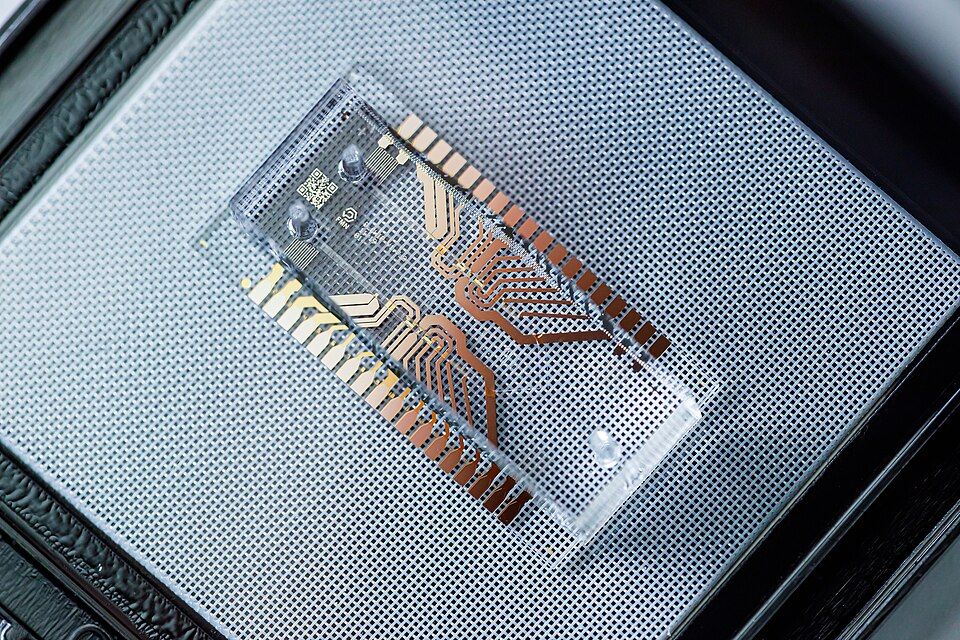
\includegraphics[width=\linewidth,height=0.45\textheight]{assets/deck-images/chip.jpg}
    \end{column}
  \end{columns}
\end{frame}

\begin{frame}[plain]
  \begin{tikzpicture}[remember picture,overlay]
    \fill[MicroCDSoft] (current page.south west) rectangle (current page.north east);
    \fill[MicroCDGreen] (current page.south west) rectangle (0.12\paperwidth,\paperheight);
  \end{tikzpicture}

  \hspace{0.9cm}
  \begin{minipage}{0.78\textwidth}
    \vspace{2.4em}
    {\footnotesize\bfseries\color{MicroCDCoral}CONTACT}

    \vspace{1.1em}
    {\Huge\bfseries MicroCD Labs}

    \vspace{0.6em}
    {\Large Microfluidics parts, equipment, and practical support for research teams.}

    \vspace{1.3em}
    Email: \texttt{info@microcdlabs.com}

    Website: \texttt{sites.google.com/view/microcd-labs/home}

    \vspace{1.3em}
    \muted{Happy to discuss lab needs, starter bundles, and research-use microfluidic supplies.}
  \end{minipage}
\end{frame}

\end{document}
